\documentclass[12pt]{article}
\usepackage[letterpaper,margin=1in]{geometry}
\usepackage{hyperref}
\usepackage{url}
\usepackage{amsmath,amssymb}
\usepackage{graphicx}
\begin{document}
\begin{center}
{\bf \LARGE AST1430 ``Cosmology'' Final}\\[7pt]
\emph{Due on Apr. 25 at 5pm}\\[7pt]
\end{center}

The full mark for the final includes the oral defense of the exercises
listed here. The breakdown is: 80\% written solutions and 20\,\% oral
defense of solutions. The points given for the different problems
below only relate to the 80\,\% written-solutions part of the full
mark.\\

This is an open-book exam, meaning that you are allowed to consult any 
resources that you wish to help you answer the questions (the slides, 
textbooks used, other online resources). However, answers should be your 
own work and distillation of the material. The final should be your own work 
and you are not allowed to consult classmates or anybody else. 
Use of chatbots like ChatGPT and similar is not allowed :-)!\\

Most of the exercises in this final must be solved on a computer
and the best way to hand in the problem set is as a \texttt{jupyter
  notebook}. Please email it to \url{mailto:jo.bovy@utoronto.ca} as an attachment. 
  \emph{Please re-run the entire notebook (with \texttt{Cell
    > Run All}) after re-starting the notebook kernel before sending it
  to me}; this will make sure that the input and output are fully
consistent.\\

If you are unfamiliar with notebooks, you can also send in a
traditional write-up (in LaTeX), but you also need to send in
well-commented code for how you solved the problems. Thus, notebooks
are strongly preferred :-)\\

\noindent{\bf Problem 1:} (20 points, 5 each) Warm up.\\

{\bf (a)} Briefly explain the motivation behind, and successes of, positing 
a brief period of inflation in the early Universe.\\

{\bf (b)} Briefly explain why the CMB is polarized.\\

{\bf (c)} Briefly explain the concept of \emph{bias} in galaxy clustering.\\

{\bf (d)} Briefly explain the evolution of large- ($k \approx 0.0001\,\mathrm{Mpc}^{-1}$)
and small-scale ($k \approx 1\,\mathrm{Mpc}^{-1}$) potential modes $\Phi(k,a)$ from the early 
Universe until today, comparing and contrasting the two.\\

%{\bf (e)} The deceleration parameter $q$ is defined as $q \equiv -\ddot{a}a/\dot{a}^2$. 
%For a matter+dark-energy FLRW Universe, work out $q(z)$ in terms of the density 
%parameters and the redshift $z$. Figure \ref{fig:sne} shows the current constraints on the 
%matter and dark-energy density parameters from the Type Ia supernovae distance-redshift 
%relation. Given that Type Ia supernovae are mainly sensitive to the deceleration parameter 
%at some redshift, determine (approximately) the redshift at which the deceleration parameter 
%is best measured from the direction of the degeneracy in the $(\Omega_M,\Omega_\Lambda)$ plane.\\
%
%\begin{figure}[t]
%    \begin{center}
%        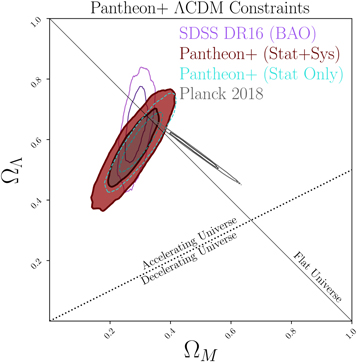
\includegraphics[width=0.5\textwidth]{apjac8e04f8_lr.jpg}
%        \caption{Cosmological constraints from the Type Ia supernovae distance-redshift relation.}
%        \label{fig:sne}
%    \end{center}
%\end{figure}

\noindent{\bf Problem 2:} (30 points, 10 each) The BAO feature in the early and late Universe.\\

One of the great advances in modern cosmology came with the measurement of the first peak in the CMB power spectrum.
In this question, you will estimate the angular size of this peak, and explore some of the implications its measurement.\\

{\bf (a)} First, we need to calculate how far acoustic waves were able to propagate through the early Universe before decoupling.
To simplify life, take the speed of sound in the primordial plasma to be $c_s = c/\sqrt{3}$, and decoupling to be instantaneous at z=1100.
Also make the (incorrect, but good enough) assumption that the Universe was matter-dominated throughout.
How far do sound waves travel before decoupling at $t \approx 340$kyr, in co-moving coordinates?
What proper distance is this at decoupling? {\it (Hint: integrate $c_s/a$ to find the co-moving distance.)}.\\

{\bf (b)} Next, we need to know how far CMB photons have travelled.
Again making the simplifying assumption that the Universe was matter-dominated throughout,
How far do CMB photos travel between t=340ky and today, t=14Gy, in co-moving coordinates?
What is the proper distance to the CMB today?\\

{\bf (c)} We measure the angular size of structures in the CMB, so scales measured are angular diameter distances.
Remembering that in a flat Universe, angular diameter distances are frozen at emission,
what angular size does the distance traversed by primordial pressure waves correspond to? Is this consistent with the observed angular scale of the first peak of the CMB?\\

\noindent{\bf Problem 3:} (50 points) Early dark energy as a solution to the $H_0$ tension.\\

We discussed in class how a cosmological model with a brief period during which a 
dark-energy-like component is important just before recombination is able to reconcile
the $H_0$ measurements from the local and inverse distance ladders. Let's explore a simple 
model for early dark energy here!

The model we consider is one in which the density parameter of the dark energy component 
is given by

\begin{equation}
    \Omega_\mathrm{de}(a) = {\Omega_{0,\mathrm{de}}-\Omega^e_\mathrm{de}\,(1-a^{-3w_0})\over \Omega_{0,\mathrm{de}}+\Omega_{0,m}\,a^{3w0}}+\Omega^e_\mathrm{de}\,(1-a^{-3w_0})\,,
\end{equation}

where $\Omega_{0,\mathrm{de}}$ is the density parameter of the dark energy component at the present day,
$\Omega_{0,m}$ is the density parameter of the matter component at the present day,
$\Omega^e_\mathrm{de}$ is the density parameter of the dark energy component in the early Universe,
and $w_0$ is the equation of state parameter of the dark energy component. This model has 
a single dark-energy component that acts as early dark energy in the early Universe and 
as late dark energy in the late Universe. We will fix $w_0=-1$ for the standard late-time dark energy model.
Reasonable values for $\Omega^e_\mathrm{de}$ are $\Omega^e_\mathrm{de} \approx 0.1$.

We will work in a spatially-flat Universe consisting of matter, radiation, and dark energy. 
We will use Planck (2018) values for the density parameters of the matter and radiation 
components, expressed as physical density parameters:

\begin{align}
    \Omega_{0,m}\,h^2 & = 0.14240\,,\\
    \Omega_{0,r}\,h^2 & = 4.12984\times 10^{-5}\,,
\end{align}

where as usual $h=H_0/(100\,\mathrm{km\,s}^{-1}\,\mathrm{Mpc}^{-1})$. We then consider two main models:

\begin{itemize}
    \item The standard $\Lambda$CDM Planck (2018) model. This model has $H_0 = 67.74\,\mathrm{km\,s}^{-1}\,\mathrm{Mpc}^{-1}$, $\Omega^e_{\mathrm{de}} = 0$. The value of $\Omega_{0,\mathrm{de}}$ is fixed through the flatness requirement, giving $\Omega_{0,\mathrm{de}} = 0.6896$. This model is in tension with the local determinations of $H_0$.
    \item A early-dark-energy model with $\Omega^e_\mathrm{de} = 0.1$ and $H_0 = 71\,\mathrm{km\,s}^{-1}\,\mathrm{Mpc}^{-1}$. This model is consistent with the local determinations of $H_0$, but let's see whether it is consistent with the CMB and the inverse distance ladder!
\end{itemize}

{\bf (a)} (5 points) Plot $\Omega_\mathrm{de}(a)$ as a function of redshift $z$ between 
$z=10^4$ and $z=0$ for the early dark-energy model.\\

{\bf (b)} (5 points) Solve for the evolution of the dark-energy density $\rho_\mathrm{de}(a)$ 
for the early dark-energy model and plot it as a function of redshift $z$ between $z=10^4$
and $z=0$. Also plot the evolution of the matter and radiation densities $\rho_m(a)$ 
and $\rho_r(a)$.\\

{\bf (c)} (5 points) Solve for the evolution of the Hubble parameter $H(a)$ for the early dark-energy 
model and plot it as a function of redshift $z$ between $z=10^4$ and $z=0$. Also compute 
the density parameters $\Omega_i(a)$ of matter, radiation, and dark energy 
and plot them as a function of redshift between $z=10^4$ and $z=0$. Discuss these results.\\

{\bf (d)} (10 points) In the early Universe ($z>10^3$), the dark energy component in the standard 
$\Lambda$CDM model is negligible and the Hubble function is given by $H^c(a)$. Demonstrate 
analytically that the Hubble function $H^e(z)$ at $z > 10^3$ in the early-dark-energy model 
when fixing all parameters aside from $\Omega^e_\mathrm{de}$
is $H^c(z)/\sqrt{1-\Omega^e_\mathrm{de}}$ and check this result numerically. Then discuss 
how the sound horizon $r_d$ at decoupling changes in the early-dark-energy model compared to 
the standard model.\\

{\bf (e)} (10 points) CMB observations determine the value of $D_M(1100)/r_d$, where $D_M(z)$ is the 
comoving angular diameter distance ($D_M(z) = c\,\int^z_0\,\mathrm{d}z/H(z)$ for a flat 
Universe). We saw in (d) that $r_d$ changes in the early-dark-energy model. Numerically 
determine how $D_M(1100)$ changes with $\Omega^e_\mathrm{de}$ for fixed $H_0$ and then 
how $D_M(1100)/r_d$ changes for reasonable values of $\Omega^e_\mathrm{de}$. Finally, 
compare $D_M(1100)/r_d$ in the two main models that we are considering and discuss.\\

{\bf (f)} (5 points) The inverse distance ladder uses BAO observations, which robustly determine 
$D_M(z)/r_d$ and $H(z)/r_d$. For $z \approx 0.5$, numerically compare the values of 
$D_M(z)/r_d$ and $H(z)/r_d$ for the two main models we are considering.\\ 

{\bf (g)} (10 points) Discuss the implications of your results for the $H_0$ tension.\\

{\bf (h)} (bonus question, 5 points) Compute the current age of the Universe $t_0$ for the two main
models we are considering. Discuss the implications of your results.\\ 


\end{document}
